%!TEX root = ../thesis.tex

\begin{subfigure}[b]{0.45\textwidth}
  \centering

  \begin{tabular}{c | c c c c}
    \m{} & $c_0$ & $c_1$ & $c_2$ & $c_3$ \\ \hline
    $s_0$ & 0 & 1 & 1 & 1 \\
    $s_1$ & 0 & 0 & 0 & 1 \\
    $s_2$ & 1 & 1 & 0 & 0 \\
    $s_3$ & 1 & 0 & 1 & 0
  \end{tabular}

  \caption{Matrix for the instance}
  \label{fig:1:a}
\end{subfigure}
\hfill
\begin{subfigure}[b]{0.45\textwidth}
  \centering

  \tikzstyle{every node}=[circle, draw]
  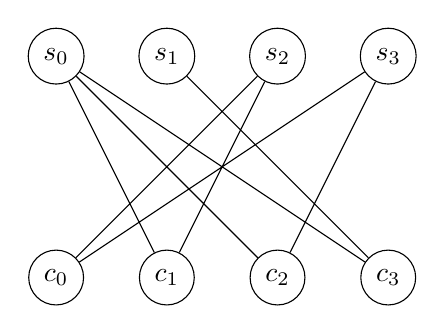
\begin{tikzpicture}
    \foreach \i in {0, ..., 3}
    {
      \path (\i*40pt, 80pt) node (s\i) {$s_{\i}$};
    }

    \foreach \j in {0, ..., 3}
    {
      \path (\j*40pt, 0) node (c\j) {$c_{\j}$};
    }

    \draw (s0) -- (c1)
          (s0) -- (c2)
          (s0) -- (c3)
          (s1) -- (c3)
          (s2) -- (c0)
          (s2) -- (c1)
          (s3) -- (c0)
          (s3) -- (c2);
  \end{tikzpicture}

  \caption{Graph for the instance}
  \label{fig:1:b}
\end{subfigure}
